% Traduction française COMIMa de l'énoncé original (anglais).
Il y a un jeton sur chaque point de la figure 1.6. En un coup, on peut déplacer simultanément deux jetons quelconques d'une place, dans des sens opposés. Le but est de réunir tous les jetons sur un même point. Quand peut-on y parvenir ?
\begin{center}
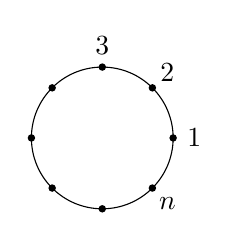
\begin{tikzpicture}[scale=0.9]
\draw (0,0) circle (1);
\foreach \a in {0,45,...,315} \fill (\a:1) circle (1.5pt);
\node at (0:1.3) {$1$}; \node at (45:1.3) {$2$}; \node at (90:1.3) {$3$}; \node at (-45:1.3) {$n$};
\end{tikzpicture}

Fig. 1.6
\end{center}
